\PassOptionsToPackage{bookmarks={true}}{hyperref}
\pdfminorversion=4
\documentclass[mathserif,xcolor={dvipsnames,table}]{beamer}
\mode<presentation>{\usetheme{Warsaw}\usecolortheme{crane}}
\usepackage{centernot}
\usepackage{upgreek}
\usepackage{graphicx}
\usepackage{geometry}
\usepackage{transparent}
\usepackage{tikz}
\usetikzlibrary{shadows}
\usepackage[utf8]{inputenc}
\usepackage[english]{babel}
\usepackage[T1]{fontenc}
\usepackage{lmodern}
\usepackage[babel=true]{microtype}
\usepackage{amsmath}
\beamertemplatenavigationsymbolsempty

\title{\textbf{Big-$\boldsymbol{\mathcal{O}}$ Ain't What it Used to Be}}
\date{}
\author{CS4803UWS at the\\
Georgia Institute of Technology
}

\begin{document}

{
\setbeamertemplate{background canvas}{%
\includegraphics[width=\paperwidth,height=\paperheight]{images/gt2.jpeg}
}%
\begin{frame}[plain]
\textcolor{white}{
\transparent{0.5}%
\colorbox{black}{\textbf{Big-$\boldsymbol{\mathcal{O}}$ Ain't What it Used to Be}}
}
\vspace{2.7in}
\\
\hfill\includegraphics[scale=.25]{images/cc-logo.pdf}

\includegraphics[scale=.25]{images/cc-new.pdf}

\includegraphics[scale=.25]{images/cc-share.pdf}
\textcolor{white}{
\\
\hfill \tiny{CC3.0 share-alike attribution}\\
}
\textcolor{white}{
\hfill \scriptsize{copyright \copyright\ 2013}\\
}
\end{frame}
}

\begin{frame}{Asymptotic notation review I}
\scriptsize{
\begin{center}
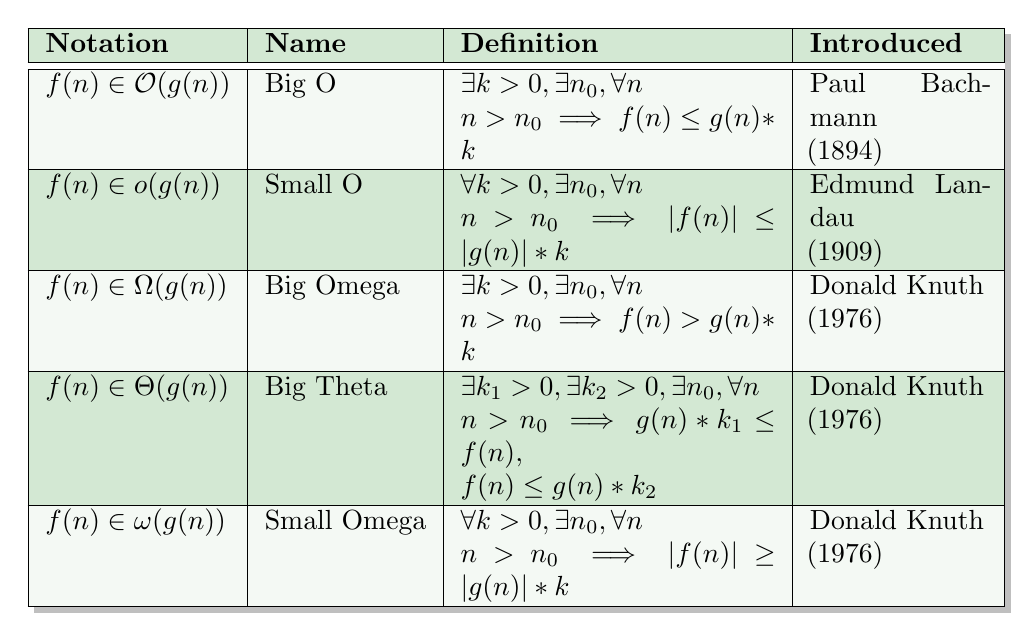
\begin{tikzpicture}
\node[drop shadow,fill=white,inner sep=0pt]
{\rowcolors{1}{ForestGreen!20}{ForestGreen!5}
\begin{tabular}{|l|l|p{4cm}|p{2.25cm}|}
\hline
\textbf{Notation} & \textbf{Name} & \textbf{Definition} & \textbf{Introduced} \\
\hline\hline
$f(n) \in \mathcal{O}(g(n))$ & Big O & $\exists k>0,\exists n_0,\forall n$
\newline
$n>n_0 \implies f(n) \le g(n)*k$ & Paul Bachmann\newline (1894) \\
\hline
$f(n) \in o(g(n))$ & Small O & $\forall k>0,\exists n_0,\forall n$
\newline
$n>n_0 \implies |f(n)| \le |g(n)|*k$ & Edmund Landau\newline (1909) \\
\hline
$f(n) \in \Omega(g(n))$ & Big Omega & $\exists k>0,\exists n_0,\forall n$
\newline
$n>n_0 \implies f(n) > g(n)*k$ & Donald Knuth\newline (1976) \\
\hline
$f(n) \in \Theta(g(n))$ & Big Theta & $\exists k_1>0,\exists k_2>0,\exists n_0,\forall n$
\newline
$n>n_0 \implies g(n)*k_1 \le f(n),
\newline
f(n) \le g(n)*k_2$ & Donald Knuth\newline (1976) \\
\hline
$f(n) \in \omega(g(n))$ &Small Omega& $\forall k>0,\exists n_0,\forall n$
\newline
$n>n_0 \implies |f(n)| \ge |g(n)|*k$ & Donald Knuth\newline(1976) \\
\hline
\end{tabular}%
};
\end{tikzpicture}
\end{center}
}
\end{frame}

\begin{frame}{Asymptotic notation review II}
\scriptsize{
\begin{center}
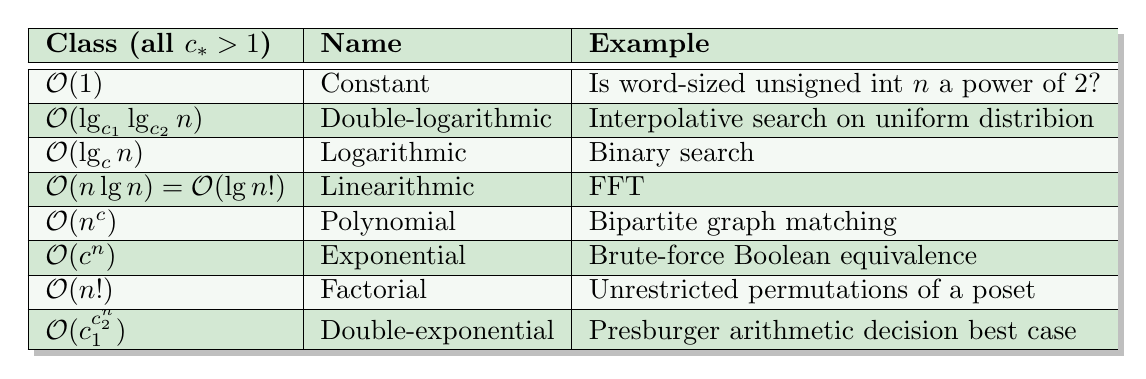
\begin{tikzpicture}
\node[drop shadow,fill=white,inner sep=0pt]
{\rowcolors{1}{ForestGreen!20}{ForestGreen!5}
\begin{tabular}{|l|l|l}
\hline
\textbf{Class (all $c_*>1$)} & \textbf{Name} & \textbf{Example} \\
\hline\hline
$\mathcal{O}(1)$ & Constant & Is word-sized unsigned int $n$ a power of 2?\\
\hline
$\mathcal{O}(\lg_{c_1}\lg_{c_2} n)$ & Double-logarithmic & Interpolative search on uniform distribion\\
\hline
$\mathcal{O}(\lg_c n)$ & Logarithmic & Binary search\\
\hline
$\mathcal{O}(n\lg n) = \mathcal{O}(\lg n!)$ & Linearithmic & FFT\\
\hline
$\mathcal{O}(n^{c})$ & Polynomial & Bipartite graph matching\\
\hline
$\mathcal{O}(c^{n})$ & Exponential & Brute-force Boolean equivalence \\
\hline
$\mathcal{O}(n!)$ & Factorial & Unrestricted permutations of a poset\\
\hline
$\mathcal{O}(c^{c^{n}_2}_1)$ & Double-exponential & Presburger arithmetic decision best case\\
\hline
\end{tabular}%
};
\end{tikzpicture}
\end{center}
}
\end{frame}

\begin{frame}{Recommended reading}
\footnotesize{
\begin{itemize}
\item Goto et al. ``Anatomy of High-Performance Matrix Multiplication'' (2008).
\item Kalyanasundaram et al. ``Improved Simulation of NTMs'' (2011).
\item FIXME
\end{itemize}
}
\end{frame}

\begin{frame}{Hack on!}
\end{frame}

\end{document}
